\documentclass[a4paper, answer, zihao = -4, unicodeGBMath, fontset=sourcesans, % sourcesans is my ctex fontset
]{ctexart}
\usepackage{danexam}
\usepackage{xpinyin}
\usepackage{adjustbox}
\usepackage{tabularx}
\newcolumntype{L}{>{$}X<{$}} % math-mode version of "l" column type


\setmainfont[Scale=1.1, SlantedFont = {Libertinus Serif Italic}]{Libertinus Serif}
\setsansfont{TeX Gyre Heros}
\setmonofont[Scale=1]{Libertinus Mono}

\begin{document}

\title{\zihao{-3}  小学二年级级质量检测\\ [-5pt]
  \zihao{-2} \heiti 语数综合试题}
\maketitle

\bigskip
{\centering
  时间:90分钟\qquad\qquad 试题95分+卷面5分=100分\par 
  \bigskip
  
  班级:\underline{\hspace{3cm}}\qquad\qquad 姓名:\underline{\hspace{4cm}} \par
}

\group{计算题。每道2分,共计12分。}

\begin{qus}
\item 直接写得数 

  \begin{tabularx}{0.9\linewidth}{*{3}{L}}
    3 \times 5 + 38 = \blankans{53}& 68-81 \div 9 = \blankans{59}& 52 \div 7 = \blankans{7 \cdots\cdots 3}\\
    6 \times 8 - 13 = \blankans{35} & 72 \div 9 \times 8 = \blankans{64}& 59 + 28 - 14 = \blankans{73}
  \end{tabularx}
\end{qus}

\group{判断题:每题1分,共计2分。对的的在题后括号内画\ding{52},错的画\ding{56}。}

\begin{qus}
\item (扁舟)中的(扁)的正确读音是\pinyin{bian3}。\cuo
\item  铁比木头重。\cuo
\end{qus}

\group{选择题:每题1分,共计2分。}

\begin{qus}

\item 土(产)——给括号中的字选择正确的解释 \choice{A}
  \begin{tasks}(2)
    \task 出自人工或天然的物品 \task 泛指房地或财物 \task 自然生长、人工制造或种
    植、出品
  \end{tasks}

\item (如)此——给括号中的字选择正确的解释 \choice{A}
  \begin{tasks}(4)
    \task 似;好像 \task 及;比得上 \task 依照 \task 如果
  \end{tasks}

\end{qus}

\group{填空题:每一空1分,共计26分。}

\begin{qus}
\item 用$4,2,0,7$这四个数字写出一个不读零的四位数是\gapline{4270},写出一个读零
  的数字是\gapline{4027}。
  
\item \adjustbox{scale=1.5}{○\symbol{"25B2}□○\symbol{"25B2}□○\symbol{"25B2}□}…………第20个图形是\gapline{△}。

  \item 小明有两件颜色不同的上衣和两条颜色不同的裤子,他可以有\gapline{4}种不同
    的穿法。

\item 有语文、数学、品德三种书,小明、小丽、小红各拿一本;小明说:“我拿的是语文
  书”。小丽说:“我拿的不是数学书”。小红拿的是\gapline{数学}书。

\item 读拼音,写词语,并选择一个词语写一句话。 % TODO: 应当提供田字格和
                                % 是否显示其中文字的命令。

  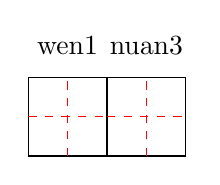
\begin{tikzpicture}[every.path/.style={red, thick}, secondary/.style={very thin, dashed,red}]
    \foreach \x in {1,...,2} {
      \draw (\x -1, 0) rectangle ++(1, 1);
      \draw[secondary] (\x - 1, 0.5) -- (\x, 0.5);
      \draw[secondary] (\x - 0.5, 0) -- (\x - 0.5, 1);
    }
    \draw (0.5,1.4) node{\pinyin{wen1}};
    \draw (1.5,1.4) node{\pinyin{nuan3}};
  \end{tikzpicture}
  \hspace{1em}
  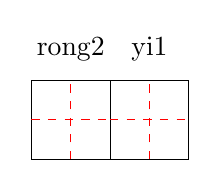
\begin{tikzpicture}[every.path/.style={red, thick}, secondary/.style={very thin, dashed,red}]
    \foreach \x in {1,...,2} {
      \draw (\x -1, 0) rectangle ++(1, 1);
      \draw[secondary] (\x - 1, 0.5) -- (\x, 0.5);
      \draw[secondary] (\x - 0.5, 0) -- (\x - 0.5, 1);
    }
    \draw (0.5,1.4) node{\pinyin{rong2}};
    \draw (1.5,1.4) node{\pinyin{yi1}};
  \end{tikzpicture}
  \hspace{1em}
  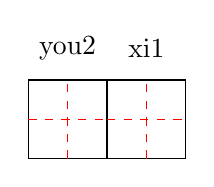
\begin{tikzpicture}[every.path/.style={red, thick}, secondary/.style={very thin, dashed,red}]
    \foreach \x in {1,...,2} {
      \draw (\x -1, 0) rectangle ++(1, 1);
      \draw[secondary] (\x - 1, 0.5) -- (\x, 0.5);
      \draw[secondary] (\x - 0.5, 0) -- (\x - 0.5, 1);
    }
    \draw (0.5,1.4) node{\pinyin{you2}};
    \draw (1.5,1.4) node{\pinyin{xi1}};
  \end{tikzpicture}
  \hspace{1em}
  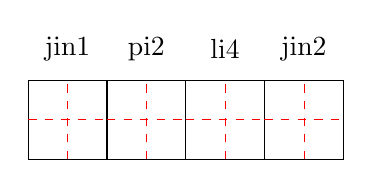
\begin{tikzpicture}[every.path/.style={red, thick}, secondary/.style={very thin, dashed,red}]
    \foreach \x in {1,...,4} {
      \draw (\x -1, 0) rectangle ++(1, 1);
      \draw[secondary] (\x - 1, 0.5) -- (\x, 0.5);
      \draw[secondary] (\x - 0.5, 0) -- (\x - 0.5, 1);
    }
    \draw (0.5,1.4) node{\pinyin{jin1}};
    \draw (1.5,1.4) node{\pinyin{pi2}};
    \draw (2.5,1.4) node{\pinyin{li4}};
    \draw (3.5,1.4) node{\pinyin{jin2}};
  \end{tikzpicture}
  \hspace{1em}
  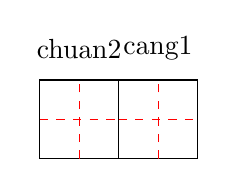
\begin{tikzpicture}[every.path/.style={red, thick}, secondary/.style={very thin, dashed,red}]
    \foreach \x in {1,...,2} {
      \draw (\x -1, 0) rectangle ++(1, 1);
      \draw[secondary] (\x - 1, 0.5) -- (\x, 0.5);
      \draw[secondary] (\x - 0.5, 0) -- (\x - 0.5, 1);
    }
    \draw (0.5,1.4) node{\pinyin{chuan2}};
    \draw (1.5,1.4) node{\pinyin{cang1}};
  \end{tikzpicture}

\item 给下面句子添加标点符号:

  “咦,是谁救了小白兔\gapline{?}”小动物们说\gapline{,}“真得谢谢他呢
  \gapline{!}”

\item 词语巧搭配。

  \gapline{翠绿}的小草 \qquad \gapline{阴凉}的树荫 \qquad \gapline{和煦}的春风

  \gapline{快活}地蹦跳 \qquad \gapline{困惑}地问\hspace{\ccwd} \qquad \gapline{委屈}地哭 
\end{qus}

\group{按要求写句子。每题4分,共计12分}
  \begin{qus}
  \item 月亮姑娘\CJKunderdot{像}一只圆盘。(用带点的词写句子)

    飘来的树叶\gapline{像是在大海里沉浮地一片片浮萍。}

  \item 雪松们拉着手,请小鸟留下歌声 。(仿写拟人句)

      \oneline{火焰欺负了蜡烛,害的蜡烛在一旁伤心得流泪。 }

  \item 例:小象\CJKunderdot{一会儿}帮主人摘果子,\CJKunderdot{一会儿}又用长长
    的鼻子往家里搬木头。(用一会儿……一会儿……造句)

    \oneline{} % TODO:应在danexam增加支持多行rulefill并可显示答案的命令

    \oneline{}

  \end{qus}

\group{问答题。每题5分,共计15分。}

\begin{qus}
  \item 我们班有26名男同学,23名女同学,按一小组最多六人来计算,全班最多可以分为几
    个小组?
    \begin{solution}[3cm]
      \begin{align*}
        26 + 23 = 49\text{(名)}
        49 \div 6 = 8 \cdots \cdots 1 \text{(个)}
      \end{align*}
      答:最多可以分为9个小组。
    \end{solution}

  \item 看图列式:
    \begin{figure}[ht]
      \centering
      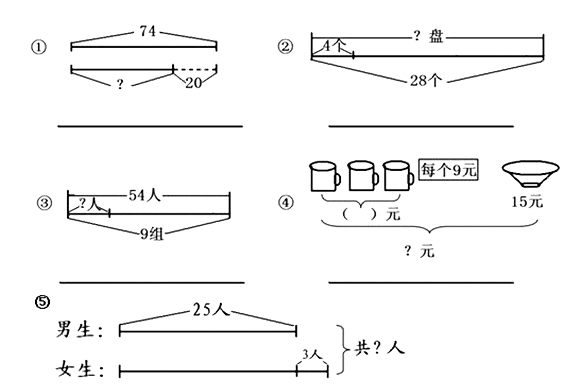
\includegraphics[width = 0.9\linewidth]{shuxue}

      \rule[-2mm]{5cm}{2pt}\hspace*{2cm}
    \end{figure}

  \item 小朋友们走路的方式很多,如唱着歌走、与小伙伴肩并肩走、踢着石头走、倒着走、
    连蹦带跳走……你喜欢怎样走路呢?走路时你是怎样的心情呢?写一写吧。
    \begin{solution}[4cm]
      
    \end{solution}
    
\end{qus}
\clearpage

\group{作文题。26分。}

\begin{qus}

\item 你最喜欢或者讨厌哪种动物?为什么喜欢或者讨厌它?自己起一个题目,写出你的理由,试着多写几条。
  
  \drawcomposition[1]{15}{15}

\end{qus}
\end{document}
